\documentclass{automatextcc}
\usepackage{ulem}
\usepackage{dsfont}
\usepackage{}

% Caminho da Pasta das Figuras
\graphicspath{{figuras/}}

%\makeindex  Opcional (Índice Remissivo)

\newcommand{\pumi}[1]{\textcolor{red}{#1}}
\newcommand{\R}{\mathds{R}}
\begin{document}


\title{Composição Automática de Músicas utilizando Redes Neurais Recorrentes}
\author{Nicolas Mathias Hahn}

% orientador(a) do trabalho {nome}{Orientador(a)}
\advisor{Prof. Dr. Guilherme Pumi}{Orientador}
% universidade onde obteve o título e atual
\advisorinfo{Doutor pela Universidade Federal do Rio Grande do Sul, Porto Alegre, RS}{UFRGS}

% banca examinadora:
\examinera{Prof. Dr. xxx}
\examinerainfo{Doutor pela XX -- Cidade, Estado}{Universidade}

% departamento:
\dept{\DEST}

% data de entrega:
\date{Outubro de 2022}


% Capa
\maketitulo

% Folha de rosto
\makefolhaderosto

% Folha de aprovação
\makefolhadeaprovacaoA % Um membro na banca
%\makefolhadeaprovacaoB % Dois membros na banca


% Epígrafe (OPCIONAL)
\newpage
\vspace*{\fill}
\begin{flushright} % mexer aqui
	\textit{``Since I have always preferred making plans to executing them, I have gravitated towards situations and systems that, once set into operation, could create music with little or no intervention on my part. That is to say, I tend towards the roles of planner and programmer, and then become an audience to the results.''} \newline
	\textit{Brian Eno \citep{alpern1995}}.
\end{flushright}

% Agradecimentos
\newpage
\chapter*{Agradecimentos}
Agradeço a xxx. Opcional % mexer aqui

% palavras chave
    % português
\keyword{Redes Neurais}
\keyword{Música}
    % inglês
\keyworde{Neural Networks}
\keyworde{Music}

% resumo 
    % português
\begin{abstract}
Este trabalho ....
\end{abstract}
    % inglês
\begin{englishabstract}
In this work ....
\end{englishabstract}

% sumário (Obrigatório)
\tableofcontents

% lista de ilustrações (Obrigatório)
\listoffigures

% lista de tabelas (Obrigatório)
\listoftables

% se um pato perde a pata, ele fica manco ou viúvo???

% Regras do PUMI:
%  * vamos ver a introdução por último
%  * deixar em bullets os itens que pretende falar
%  * focar na fundamentação teórica (redes neurais, RNN e LSTM)


%%%%%%%%%%%%%%%%%%%%%%%%%%%%%%%%%%%
%%%%  Introdução
%%%%%%%%%%%%%%%%%%%%%%%%%%%%%%%%%%%
\chapter{Introdução}

\begin{itemize}
    \item composição algorítmica (composição automática) - caminhar histórico?
    \item formas de composição algorítmica: rule-based, stochastic e AI
\end{itemize}

% certamente olhar este artigo e suas bibliografias:
% https://ccrma.stanford.edu/~blackrse/algorithm.html

% talvez olhar este artigo:
% https://musica.ufmg.br/nasnuvens/wp-content/uploads/2020/11/2016-38-A-interatividade-nas-trilhas-sonoras-de-jogos-digitais-e-um-comparativo-com-a-música-de-cinema.pdf



% referencial teórico
\chapter{Referencial Teórico}

    % NN
\section{Redes Neurais Artificiais}
    % aggarwal 2018
%Redes Neurais Artificiais são técnicas populares de aprendizagem de máquina que simulam o mecanismo de aprendizagem presente em organismos vivos.
    % haykin 2002
%O trabalho em redes neurais artificiais, usualmente denominadas "redes neurais", tem sido motivado desde o começo pelo reconhecimento de que o cérebro humano processa informações de uma forma diferente do computador digital convencional. O cérebro é um computador (sistema de processamento de informação) altamente complexo, não linear e paralelo. Ele tem a capacidade de organizar seus constituintes estruturais, conhecidos por neurônios, de forma a realizar certos processamentos (ex. reconhecimento de padrões, percepção e controle motor) muito mais rapidamente que o mais rápido computador digital hoje existente.
    % elements of statistical learning 2008
%O termo "rede neural" tem evoluído para abranger uma grande classe de modelos e métodos de aprendizagem. [...] Elas são apenas modelos estatísticos não lineares.
    % goodfellow 2016
%Alguns dos algoritmos iniciais que reconhecemos hoje tinham o intuito de ser um modelo computacional da aprendizagem biológica, i.e., modelos de como a aprendizagem poderia ocorrer no cérebro. A correspondente perspectiva de deep learning (redes neurais artificiais) é que são engineered systems inspirados pelo cérebro (seja humano seja de outro animal)
    % hair et al 2005
%Redes neurais são uma abordagem totalmente diferente para a análise de dados em relação a qualquer outra técnica multivariada. Em vez de conceitualizar o problema como de caráter matemático, redes neurais usam o cérebro humano e sua estrutura para desenvolver uma estratégia de processamento. Apesar de jamais sermos capazes de construir redes neurais tão complexas quanto o cérebro humano, podemos usar seus princípios básicos de unidades de processamento paralelo múltiplo engajadas no reconhecimento de padrões. 

% paragrafo
Redes Neurais Artificiais (RNA) são técnicas de aprendizagem de máquina que simulam o mecanismo de aprendizagem presente em organismos vivos \citep{aggarwal2018}. Em \citet{goodfellow2016} é comentado que os algoritmos iniciais tinham o intuito de ser um modelo computacional de como a aprendizagem poderia ocorrer no cérebro (seja humano seja de outro animal). O cérebro, expressa \citet{haykin2001}, é um computador (sistema de processamento de informação) altamente complexo, não linear e paralelo. Por fim, RNAs podem ser vistas como modelos estatísticos não lineares \citep{hastie2009}.

\subsection{Deep Learning}

\begin{itemize}
    \item renascimento de redes neurais 
    \item deep learning são redes neurais profundas (com muuuitas camadas)
\end{itemize}


\subsection{Redes Neurais e a Estatística}
Muitos modelos de RNAs são similares ou idênticos a populares técnicas estatísticas como modelos lineares generalizados, regressão linear (simples e múltipla), regressão polinomial, regressão não paramétrica e análise discriminante (como a regressão logística) entre outros, especialmente quando a ênfase é na predição de um fenômeno complexo em vez de sua explicação \citep{sarle1994, cheng1994}.

No contexto de RNAs, dois aspectos de tratamento podem ser definidos a um problema prático: (i) especificar a arquitetura da rede; (ii) treinar a rede para performar bem com o conjunto de treinamento (referencial). Para o estatístico, tais passos são equivalentes a: (i) especificar um modelo de regressão; (ii) estimar os parâmetros do modelo dado um conjunto de dados \citep{cheng1994}.


\subsubsection{Jargões} 
Apesar de muitos modelos de RNAs serem similares ou idênticos aos modelos estatísticos, os termos na literatura de RNAs são bastante diferentes da estatística:

\begin{itemize}
    \item variables are called features
    \item independent variables are called input
    \item predicted values are called output
    \item dependent variables are called targets or training values
    \item residuals are called errors
    \item estimation is called training, learning, adaptation, or selforganization
    \item an estimation criterion is called an error function, cost function, or Lyapunov function
    \item observations are called patterns or training pairs
    \item parameter estimates are called (synaptic) weights
    \item interactions are called higher-order neurons
    \item transformations are called functional links
    \item regression and discriminant analysis are called supervised learning or heteroassociation
    \item data reduction is called unsupervised learning, encoding, or autoassociation
    \item cluster analysis is called competitive learning or adaptative vector quantization
    \item interpolation and extrapolation are called generalization
\end{itemize}
Os termos estatísticos amostra e população não demonstram conter equivalentes na literatura de RNAs. No entanto, os dados são comumentes dividos em conjunto de treino e de teste para validação cruzada \citep{cheng1994}.


\subsection{Neurônio}
Um neurônio (ou nó computacional) é uma unidade de processamento de informação fundamental para a operação de uma rede neural \citep{haykin2001}. Podemos identificar três elementos básicos do modelo neuronal:
\begin{enumerate}
    \item Um conjunto de sinapses, cada uma caracterizada por um peso ou força própria. O peso sináptico de um neurônio artificial pode estar em um intervalo que inclui valores positivos e negativos.
    \item Um \textit{somador} ou \textit{acumulador} para somar os sinais de entrada, ponderados pelas respectivas sinapses de cada neurônio, constituindo uma \textit{combinação linear}.
    \item Uma \textit{função de ativação} para restringir a amplitude de saída de um neurônio (fixando em um valor finito).
\end{enumerate}
Também é incluído um \textit{bias} (viés) no modelo, externo ao neurônio, com o intuito de aumentar ou diminuir a entrada da função de ativação, dependendo do seu sinal.

Matematicamente, podemos descrever um neurônio $k \in \mathds{N}$, por meio de um par de equações:
\begin{align*}
    y_k &= \varphi(u_k + b_k) = \varphi(v_k);\\[.2cm]
    u_k &= \displaystyle{\sum_{i=1}^{m} }w_{k,i}x_i;
\end{align*}
em que $x_i \in \R$, $i \in \{1,\dots,m\}$, $m \in \mathds{N}$, são os valores observados; $w_{k,i} \in \R$, são os pesos associados ao neurônio $k$; $u_k$ é a saída da combinação linear entre os sinais de entrada e os pesos; $b_k$ é o \textit{bias}; $\varphi(\cdot)$ é uma função de ativação; e $y_k$ é o sinal de saída.

\begin{figure}
    \centering
    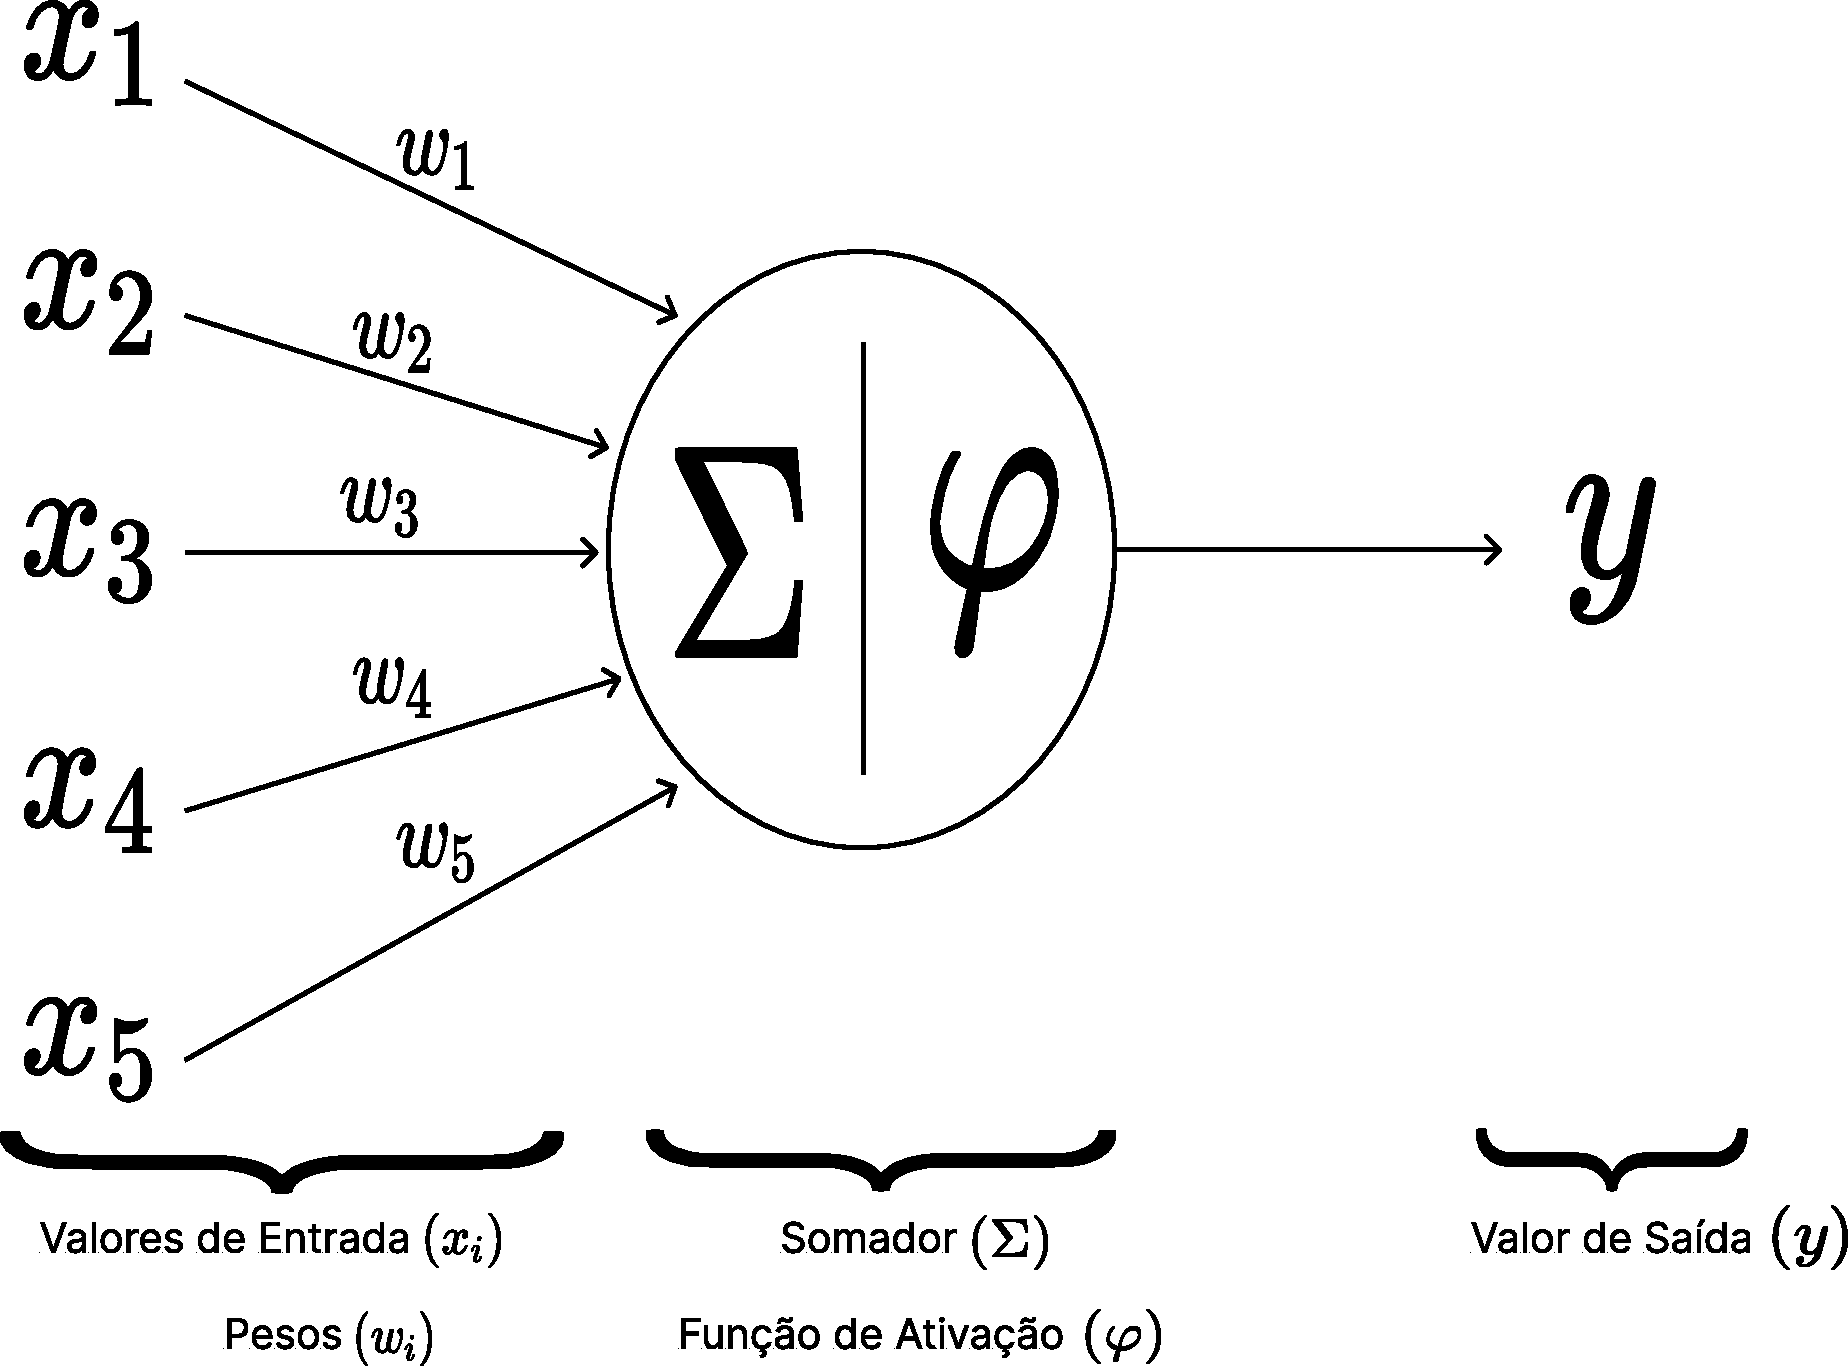
\includegraphics[width=10cm,height=8cm]{figuras/neuron_model.pdf}
	\caption{Modelo Neuronal (adaptado de \citet{haykin2001,hair2005})}
\end{figure}

\subsection{Função de Ativação}
O objetivo da função de ativação (ou de transferência) é determinar se a informação que o neurônio está recebendo será passada adiante ou será ignorada \citep{dsa2022}. \citet{hagan2014} comenta que uma função de ativação particular é selecionada para satisfazer uma determinada especificação do problema que o neurônio almeja resolver. Assim, temos que a função de ativação pode ser linear ou não-linear. Abaixo, seguem algumas funções de ativação:

\begin{itemize}
    \item \textbf{linear:} $f: \R \rightarrow \R$ dada por $f(x) = \alpha x,$  $\alpha \in \R\backslash\{0\}$. Observe que no caso da função linear, o neurônio está sempre ativado, sendo seu valor alterado pela constante $\alpha$. Em particular, quando $\alpha=1$, temos a função identidade e, como comenta \citet{sarle1994}, um modelo de regressão linear.
    \item \textbf{sigmóide ou \textit{logit}}: $f: \R \rightarrow (0,1)$ dada por $f(x) = \frac{1}{1 + e^{-x}}$. Quando a rede tem essa função de ativação, o neurônio é um modelo linear generalizado conhecido como regressão logística. Dessa forma, notamos que a função de ativação tem um papel semelhante à função de ligação: relacionar o preditor linear $v$ a um valor esperado $\mu$ de um dado $y$ \citep{sarle1994,frei2020,mccullagh1989}.
    \item \textbf{tangente hiperbólica (\textit{tanh}):}  $f:\R \rightarrow (-1,1)$ dada por $f(x) = \frac{e^{x}-e^{-x}}{e^{x}+e^{-x}}$. Em contextos que uma função sigmoidal é necessária (como a predição de uma variável binária), a \textit{tanh} tipicamente performa melhor. Vale comentar que funções de ativação sigmoidal são mais comuns em estruturas diferentes que a de redes alimentadas adiante, como as redes recorrentes \citep{goodfellow2016}.  
    \item \textbf{ReLU (\textit{Rectified Linear Unit}):} $f: \R \rightarrow [0,\infty)$ dada por $f(x) = \max\{0,x\}$. De acordo com \citet{goodfellow2016}, é a recomendação padrão para redes neurais modernas. O autor justifica que, por ser uma função quase linear, são preservadas muitas propriedades que fazem os modelos linear bons generalizadores. % pq? % quais? 
\end{itemize}

% pq domínio é igual para todos?

Listas de funções de ativação comumente utilizadas podem ser encontradas em \citet{hagan2014}, \citet{aggarwal2018} e \citet{dsa2022}.


\subsection{Arquitetura de RNAs}
%Comumente, um neurônio, mesmo com muitas entradas, pode não ser suficiente. Talvez sejam necessários cinco ou dez, operando paralelamente, no que chamamos de ``camada'' \citep{hagan2014}.  
%Em geral, podemos identificar três classes de arquiteturas de rede fundamentalmente diferentes \citep{haykin2001}.

\citet{hagan2014} afirma que um neurônio, mesmo com muitas entradas, usualmente não é suficiente, sendo necessários cinco ou dez operando paralelamente, em uma estrutura que chamamos de ``camada''. Devido a isso, organizamos as redes em três arquiteturas fundamentalmente diferentes \citep{haykin2001}.



% inteira retirada de haykin_2001 (apenas copiado)
\subsubsection{Redes Alimentadas Adiante com Camada Única | Perceptron?}
Em uma rede neural em camadas, os neurônios estão organizados na forma de camadas. Na forma mais simples de uma rede em camadas, temos a camada de entrada de nós de fonte que se projeta sobre uma camada de saída de neurônios (nós computacionais), mas não vice-versa. Em outras palavras, esta rede é estritamente do tipo alimentada adiante ou acíclica. [...]. Esta rede é chamada de camada única sendo que a designação ``camada única'' se refere à camada de saída de nós computacionais (neurônios). Não contamos a camada de entrada de nós de fonte, porque lá não é realizada nenhuma computação.

\subsubsection{Redes Alimentadas Diretamente com Múltiplas Camadas | MLP | Feedforward}
A segunda classe de uma rede neural alimentada se distingue pela presença de uma ou mais camadas ocultas, cujos nós computacionais são chamados correspondentemente de neurônios ocultos ou unidades ocultas. A função dos neurônios ocultos é intervir entre a camada externa e a saída da rede de uma maneira útil. Adicionando-se uma ou mais camadas ocultas, tornamos a rede capaz de extrair estatísticas de ordem elevada. Em um sentido bastante livre, a rede adquire uma perspectiva global apesar de sua conectividade local, devido ao conjunto extra de conexões sinápticas e da dimensão extra de interações neurais (Churland e Sejnowski, 1992). A habilidade de os neurônios ocultos extraírem estatísticas de ordem elevada é particularmente valiosa quando o tamanho da camada de entrada é grande.

Os nós de fonte da camada de entrada da rede fornecem os respectivos elementos do padrão de ativação (vetor de entrada), que constituem os sinais de entrada aplicados aos neurônios (nós computacionais) na segunda camada (i.e., primeira camada oculta). Os sinais de saída da segunda camada são utilizados como entradas para a terceira camada, e assim por diante para o resto da rede. Tipicamente, os neurônios em cada camada da rede têm como suas entradas apenas os sinais de saída da camada precedente. O conjunto de sinais de saída (final) da rede constitui a resposta global da rede para o padrão de ativação fornecido pelos nós de fonte da camada de entrada (primeiro). [...]. Como um outro exemplo, uma rede alimentada adiante com $m$ nós de fonte, $h_1$ neurônios na primeira camada oculta, $h_2$ neurônios na segunda camada oculta e $q$ neurônios na camada de saída é referida como uma rede $m-h_1-h_2-q$.

A rede neural é dita totalmente conectada, no sentido de que cada um dos nós de uma camada da rede está conectado a todos os nós da camada adjacente seguinte. Entretanto, se alguns dos elos de ligação (conexões sinápticas) estiverem faltando na rede, dizemos que a rede é parcialmente conectada.

\subsubsection{Redes Neurais Recorrentes}
Uma rede neural recorrente se distingue de uma rede neural alimentada adiante por ter pelo menos um laço de realimentação. Uma rede recorrente pode consistir, por exemplo, de uma única camada de neurônios com cada neurônio alimentando seu sinal de volta para as entradas de todos os outros neurônios. [...]; auto-realimentação se refere a uma situação onde a saída de um neurônio é realimentada para a sua própria entrada. [...].

A presença de laços de realimentação, [...], tem um impacto profundo na capacidade de aprendizagem da rede e no seu desempenho. Além disso, os laços de realimentação envolvem o uso de ramos particulares compostos de elementos de atraso unitário (representado por $z^{-1}$, o que resulta em um comportamento dinâmico não-linear, admitindo-se que a rede contenha unidades não-lineares.

\section{Composição Algorítmica | Composição Musical}

\begin{itemize}
    \item composição algorítmica ou automática
    \item como já foi explorado o processo de composição de forma mais automática
\end{itemize}

\section{Web Crawler | Web Scrapper}

\begin{itemize}
    \item coleta de dados online
    \item o que é um bot
\end{itemize}

\section{Estatística | Machine Learning}

\begin{itemize}
    \item modelos estatísticos (glm por exemplo)
    \item problemas de regressão e classificação (nomenclatura machine learning)
\end{itemize}


%%%%%%%%%%%%%%%%%%%%%%%%%%%%%%%%%%%
%%%%  Metodologia
%%%%%%%%%%%%%%%%%%%%%%%%%%%%%%%%%%%
\chapter{Metodologia}

% coleta de dados
\section{Coleta de Dados}

% resumo como foram coletados os dados (fonte também) e que isso resultou em error 403 (acesso negado) no site hehe

A coleta de dados foi realizada por meio de um \textit{crawler/bot}, desenvolvido na linguagem \href{https://python.org/}{Python}, para extrair músicas em formato \textit{.abc} do site \href{https://abcnotation.com/}{``abcnotation.com''}. Após uma semana de execução, foram obtidos 184.900 arquivos contendo diversas informações sobre as peças musicais (como título, autor, tonalidade, entre outras).

% tratamento de dados
\section{Tratamento de Dados}

% explicar a forma que tratei os arquivos .abc:
%   - removi títulos
%   - removi letras das músicas
%   - removi caracteres de comentários
%   - codifiquei/vetorizei as strings para que fosse possível ir e vir (caractere --> index e vice-versa)

% rede neural
\section{Rede Neural}
    % arquitetura
\subsection{Arquitetura}
    % parâmetros de treinamento
\subsection{Parâmetros de Treinamento}

%%%%%%%%%%%%%%%%%%%%%%%%%%%%%%%%%%%
%%%%  Resultados
%%%%%%%%%%%%%%%%%%%%%%%%%%%%%%%%%%%
\chapter{Resultados}

% trocar função de ativação (mesma semente)
% treinar rede apenas com mesma tonalidade (ou algo assim)
% retirar músicas no treino, o quanto que muda o resultado final

%%%%%%%%%%%%%%%%%%%%%%%%%%%%%%%%%%%
%%%%  Conclusão
%%%%%%%%%%%%%%%%%%%%%%%%%%%%%%%%%%%
\chapter{Conclusão}

%%%%%%%%%%%%%%%%%%%%%%%%%%%%%%%%%%%
%%%%  Referências
%%%%%%%%%%%%%%%%%%%%%%%%%%%%%%%%%%%
\addcontentsline{toc}{chapter}{Referências Bibliográficas} % Coloca no sumário
\bibliographystyle{apalike-br}
\bibliography{biblio}


%\printindex % Opcional  Índice remissivo

\end{document}
